\fenicschapter{Tensor Representation of Finite Element Variational Forms}
              {Tensor Representation of Finite Element Variational Forms}
              {Robert C. Kirby and Anders Logg}
              {kirby-8}

In Chapter~[logg-3], we saw that an important step in the assembly of
matrices and vectors for discretization of finite element variational
problems is the evaluation of the element (cell) tensor $A_T$ defined
by
\begin{equation*}
  A_{T,i}
  = a_T(\phi^{T,1}_{i_1}, \phi^{T,2}_{i_2}, \ldots, \phi^{T,\rho}_{i_{\rho}}).
\end{equation*}
Here, $a_T$ is the local contribution to a multilinear form $a:
V^1 \times V^2 \times \cdots \times V^{\rho}$, $i$ is a multiindex of
length~$\rho$, and $\{\phi^{T,j}_{i_j}\}$ is a basis for the local
finite element space of $V^j_h \subset V^j$ on a local cell~$T$. In
this chapter, we describe how the cell tensor~$A_T$ can be computed
efficiently by an approach referred to as tensor representation.

%------------------------------------------------------------------------------
\section{Tensor Representation for Poisson's Equation}

We first describe how one may express the element tensor for Poisson's
equation as a special tensor contraction and explain below how this
may be generalized to other variational forms. For Poisson's equation,
the element tensor (matrix) $A_T$ is defined by
\begin{equation*}
  A_{T,i} =
  \int_T
  \nabla \phi_{i_1}^{T,1} \cdot
  \nabla \phi_{i_2}^{T,2} \dx
  =
  \int_T
  \sum_{\beta=1}^d
  \frac{\partial \phi_{i_1}^{T,1}}{\partial x_{\beta}}
  \frac{\partial \phi_{i_2}^{T,2}}{\partial x_{\beta}} \dx.
\end{equation*}
Let $F_T : T_0 \rightarrow T$ be an affine map from a reference
cell~$T_0$ to the current cell~$T$ as illustrated in
Figure~\ref{fig:affinemap}. Using this affine map, we make a change of
variables to obtain
\begin{equation}
  A_{T,i} =
  \int_{T_0}
  \sum_{\beta=1}^d
  \sum_{\alpha_1=1}^d
  \frac{\partial X_{\alpha_1}}{\partial x_{\beta}}
  \frac{\partial \Phi^1_{i_1}}{\partial X_{\alpha_1}}
  \sum_{\alpha_2=1}^d
  \frac{\partial X_{\alpha_2}}{\partial x_{\beta}}
  \frac{\partial \Phi^2_{i_2}}{\partial X_{\alpha_2}}
  \det F_T'
  \dX.
\end{equation}
Here, $\Phi_i^j = \phi_i^{T,j} \circ F_T$ denotes the basis function
on the reference cell~$T_0$ corresponding to the basis function
$\phi_i^{T,j}$ on the current cell~$T$. Since $F_T$ is affine, the
derivatives $\partial X / \partial x$ and the determinant~$\det F_T'$
are constant. We thus obtain
\begin{equation}
  A_{T,i} =
  \det F_T'
  \sum_{\alpha_1=1}^d
  \sum_{\alpha_2=1}^d
  \sum_{\beta=1}^d
  \frac{\partial X_{\alpha_1}}{\partial x_{\beta}}
  \frac{\partial X_{\alpha_2}}{\partial x_{\beta}}
  \int_{T_0}
  \frac{\partial \Phi^1_{i_1}}{\partial X_{\alpha_1}}
  \frac{\partial \Phi^2_{i_2}}{\partial X_{\alpha_2}}
  \dX
  =
  \sum_{\alpha_1=1}^d
  \sum_{\alpha_2=1}^d
  A^0_{i\alpha} G_T^{\alpha},
\end{equation}
where
\begin{equation} \label{eq:poisson,AandG}
  \begin{split}
    A^0_{i\alpha}
    &=
    \int_{T_0}
    \frac{\partial \Phi^1_{i_1}}{\partial X_{\alpha_1}}
    \frac{\partial \Phi^2_{i_2}}{\partial X_{\alpha_2}}
    \dX, \\
    G_T^{\alpha}
    &=
    \det F_T'
    \sum_{\beta=1}^d
    \frac{\partial X_{\alpha_1}}{\partial x_{\beta}}
    \frac{\partial X_{\alpha_2}}{\partial x_{\beta}}.
  \end{split}
\end{equation}
We refer to the tensor~$A^0$ as the \emph{reference tensor} and to the
tensor~$G_T$ as the \emph{geometry tensor}. We may thus express the
computation of the element tensor~$A_T$ for Poisson's equation as the
tensor contraction
\begin{equation*}
  A_T = A^0 : G_T.
\end{equation*}

\begin{figure}[htbp]
  \begin{center}
    %\psfrag{p0}{$X^1 = (0,0)$}
    %\psfrag{p1}{$X^2 = (1,0)$}
    %\psfrag{p2}{$X^3 = (0,1)$}
    %\psfrag{xi}{$X$}
    %\psfrag{x}{$x = F_T(X)$}
    %%\psfrag{F=}{$F_K(X) = x^1 \Phi_1(X) + x^2 \Phi_2(X) + x^3 \Phi_3(X)$}
    %\psfrag{F=}{}
    %\psfrag{F}{$F_T$}
    %\psfrag{x0}{$x^1$}
    %\psfrag{x1}{$x^2$}
    %\psfrag{x2}{$x^3$}
    %\psfrag{K0}{$T_0$}
    %\psfrag{K}{$T$}
    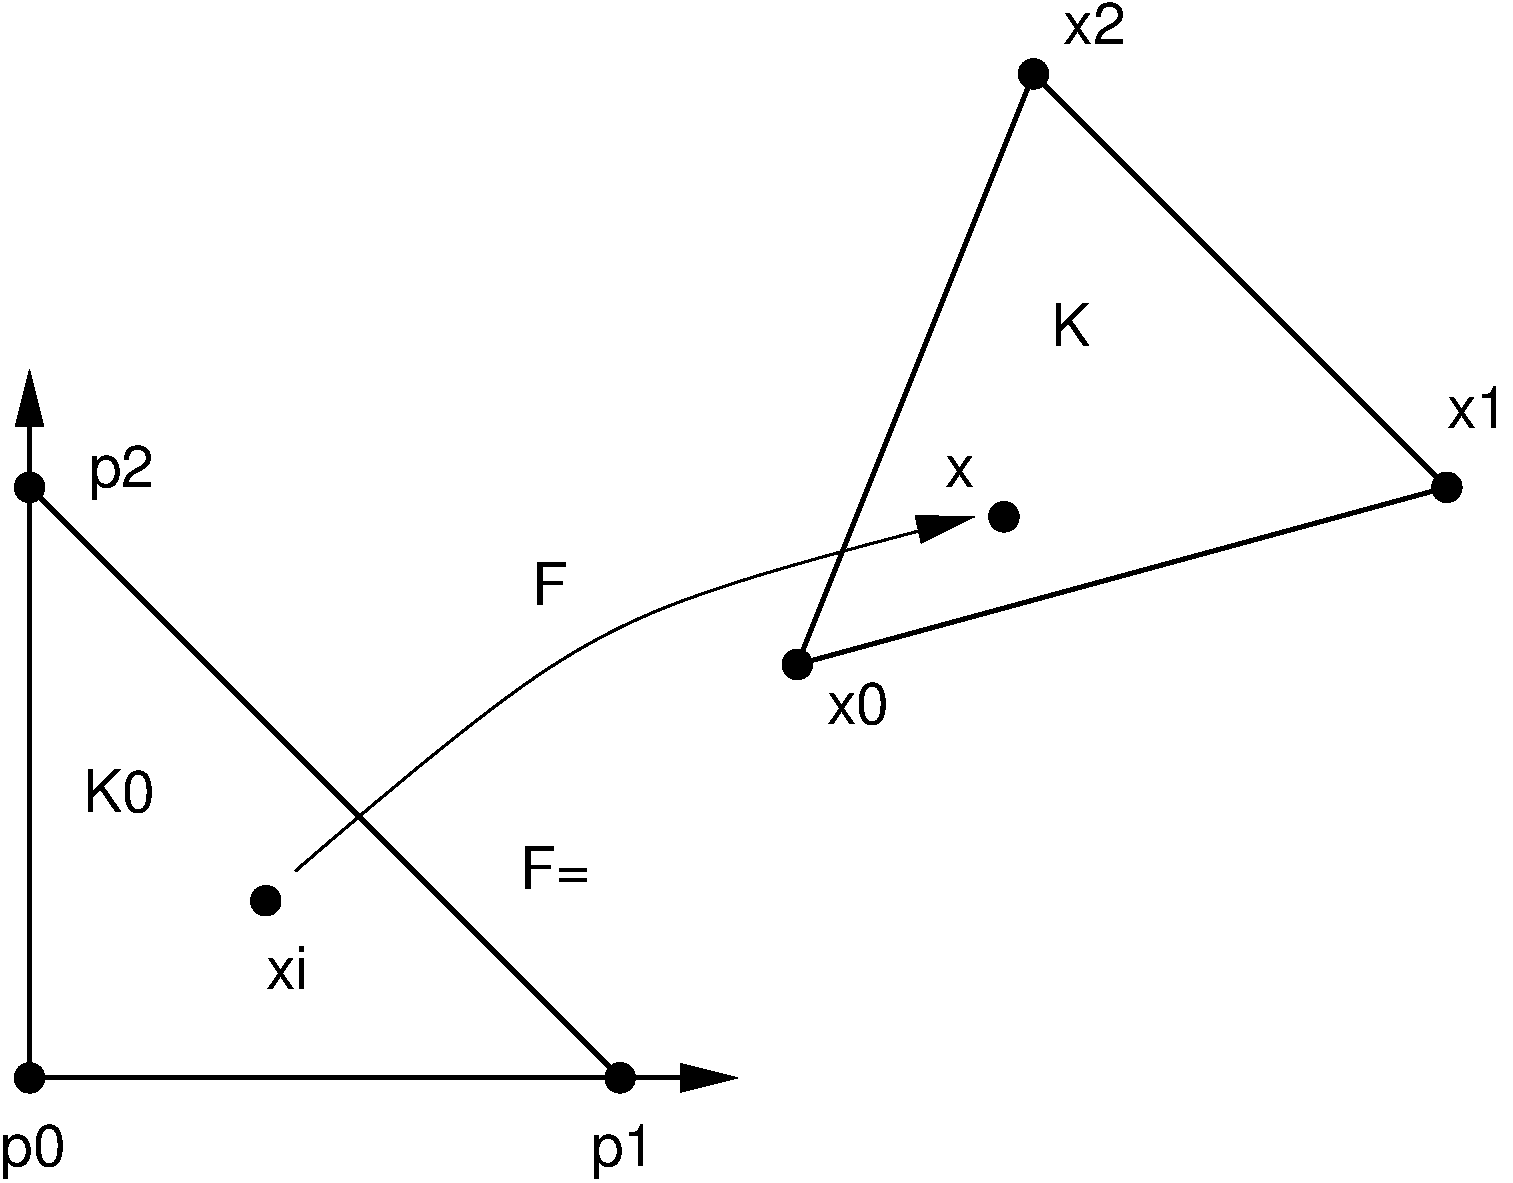
\includegraphics[width=12cm]{chapters/kirby-8/pdf/affinemap.pdf}
    \caption{The (affine) map $F_T$ from a reference cell $T_0$
      to a cell $T \in \mathcal{T}$.}
    \label{fig:affinemap}
  \end{center}
\end{figure}

This tensor contraction may be computed efficiently by precomputing
the entries of the reference tensor~$A^0$. This is possible since the
reference tensor is constant and does not depend on the cell~$T$ or
the mesh~$\mathcal{T} = \{T\}$. On each cell~$T \in \mathcal{T}$, the
element tensor may thus be computed by first computing the geometry
tensor~$G_T$ and then contracting it with the precomputed reference
tensor. In Chapter~[logg-1], we describe the FEniCS Form
Compiler~(FFC) which precomputes the reference tensor~$A^0$ at
compile-time and generates code for computing the tensor contraction.

For Poisson's equation in two space dimensions, the tensor contraction
involves contracting the $2 \times 2$ geometry tensor~$G_T$ with each
corresponding block of the reference tensor~$A^0$ to form each entry
of the element tensor $A^T$. Each of these entries may thus be
computed in only four multiply-add pairs (plus the cost of computing
the geometry tensor). This brings a considerable speedup compared to
evaluation by run-time quadrature, in particular for higher-order
elements. In Chapter~[kirby-4], we discuss how this may be improved
further by examining the structure of the reference tensor~$A^0$ to
find a reduced-arithmetic computation for the tensor contraction.

%------------------------------------------------------------------------------
\section{A Representation Theorem}

In~\cite{KirbyLogg2006}, it was proved that the element tensor for any
affinely mapped monomial multilinear form may be expressed as a tensor
contraction $A_T = A^0 : G_T$, that is,
\begin{equation*}
  A_{T,i} = \sum_{\alpha} A^0_{i\alpha} G_T^{\alpha}.
\end{equation*}
More precisely, element tensor may be expressed as a sum of tensor
contractions,
\begin{equation} \label{eq:tensorcontraction}
  A_T = \sum_k A^{0,k} : G_{T,k}.
\end{equation}
By a monomial multilinear form, we here mean a multilinear form that
can be expressed as a sum of monomials, where each monomial is a
product of coefficients, test/trial function and their derivatives.
This class covers all forms that may be expressed by addition,
multiplication and differentiation. Early versions of the form
compiler FFC implemented a simple form language that was limited to
these three operations. This simple form language is now replaced by
the new and more expressive UFL form language

The representation theorem was later extended to Piola-mapped elements
in~\cite{RognesKirbyLogg2009}, and in~\cite{OlgaardLoggWells2008} it was
demonstrated how the tensor representation may be computed for
discontinuous Galerkin methods.

The ranks of the reference and geometry tensors are determined by the
multilinear form~$a$, in particular by the number of coefficients and
derivatives of the form. Since the rank of the element tensor $A_T$ is
equal to the arity~$\rho$ of the multilinear form~$a$, the rank of the
reference tensor~$A^0$ must be $|i\alpha| = \rho + |\alpha|$, where
$|\alpha|$ is the rank of the geometry tensor. For Poisson's equation,
we have $|i\alpha| = 4$ and $|\alpha| = 2$. In Tables~\ref{tab:mass}
and~\ref{tab:advection}, we demonstrate how the tensor representation
may be computed for the bilinear forms $a(v, u) = \inner{v}{u}$ (mass
matrix) and $a(v, u) = \inner{v}{w \cdot \nabla u}$ (advection).

\begin{table}[htbp]
  \begin{center}
    \linespread{2.0}
    \begin{tabular}{|rcl|c|}
      \hline
      $a(v, u)$ &$=$& $\inner{v}{u}$ & rank \\
      \hline
      \hline
      $A^0_{i\alpha}$ &$=$& $\int_{T_0} \Phi_{i_1}^{1} \Phi_{i_2}^{2} \dX$
      & $|i\alpha| = 2$ \\
      \hline
      $G_T^{\alpha}$ &$=$& $\det F_T'$
      & $|\alpha| = 0$ \\
      \hline
    \end{tabular}
    \linespread{1.0}
    \caption{Tensor representation $A_T = A^0 : G_T$ of the element
      tensor~$A_T$ for the bilinear form associated with a mass
      matrix.}
    \label{tab:mass}
  \end{center}
\end{table}

\begin{table}[htbp]
  \begin{center}
    \linespread{2.0}
    \begin{tabular}{|rcl|c|}
      \hline
      $a(v, u)$ &$=$& $\inner{v}{w \cdot \nabla u}$ & rank \\
      \hline
      \hline
      $A^0_{i\alpha}$ &$=$&
      $\sum_{\beta=1}^d
      \int_{T_0}
      \Phi^1_{i_1}[\beta]
      \frac{\partial \Phi^2_{i_2}[\beta]}{\partial X_{\alpha_3}}
      \Phi^3_{\alpha_1}[\alpha_2]
      \dX$
      & $|i\alpha| = 5$ \\
      \hline
      $G_T^{\alpha}$ &$=$&
      $w^T_{\alpha_1} \det F_T'
      \frac{\partial X_{\alpha_3}}{\partial x_{\alpha_2}}$
      & $|\alpha| = 3$ \\
      \hline
    \end{tabular}
    \linespread{1.0}
    \caption{Tensor representation $A_T = A^0 : G_T$ of the element
      tensor~$A_T$ for the bilinear form associated with advection $w
      \cdot \nabla u$. It is assumed that the velocity field $w$ may
      be interpolated into a local finite element space with expansion
      coefficients~$w^T_{\alpha_1}$.}
    \label{tab:advection}
  \end{center}
\end{table}

%------------------------------------------------------------------------------
\section{Extensions and limitations}

The tensor contraction~\eqref{eq:tensorcontraction} assumes that the
map~$F_T$ from the reference cell is affine, allowing the transforms
$\partial X / \partial x$ and the determinant to be pulled out of the
integral. For higher-order maps, one may expand the map in the basis
functions of the corresponding finite element space (which is equal to
the test/trial spaces for isoparametric maps) and pull the
coefficients outside of the integral as for the advection term from
Table~\ref{tab:advection}. Alternatively, one may evaluate the element
tensor by quadrature and express the summation over quadrature points
as a tensor contraction as explained in~\cite{KirbyLogg2006}.  As
noted above, the tensor contraction readily extends to basis functions
mapped by Piola transforms.

One limitation of this approach is it requires each basis function on
a cell \( T \) to be the image under affine of Piola transformation of
a single reference-element basis function.  While this covers a wide
range of commonly-used elements, it does not include certain kinds of
elements with derivative-based degrees of freedom such as the Hermite
and Argyris elements.  Let \( \mathcal{F}_T \) be the mapping of the
reference element function space to the physical element space, such
as affine pullback or Piola transform.  Then, for these elements, the
physical element basis functions are expressed as a linear combination
of the transformed reference element basis functions,
\begin{equation}
\phi^T_i = \sum_{j=1}^N M_{T,{ij}} \mathcal{F}_T \left( \Phi_j \right).
\end{equation}
The structure of this matrix \( M_T \) depends on the kinds of degrees
freedom, and the values typically vary for each \( T \) based on the
cell geometry.  It is frequently sparse.  Given \( M_T \), the
tensor-contraction framework may be extended to handle these more
general elements.  As before, one may compute the reference tensor \(
A^0 \) by mapping the reference element basis functions, but in
addition the product \( A^0 : G_T \) must be corrected by acting on it
with the matrices \( M_T \). This is currently not implemented in the
form compiler FFC and thus FEniCS does not support Hermite and Argyris
elements.

For many simple variational forms, such as those for Poisson's
equation, the mass matrix and the advection term discussed above, the
tensor contraction~\eqref{eq:tensorcontraction} leads to significant
speedups, sometimes several orders of magnitude, over evaluation by
quadrature. However, as the complexity of a form increases, the
relative efficiency of quadrature also increases. In simple terms, the
complexity of a form can be measured as the number of derivatives and
the number of coefficients appearing in a form. For each derivative
and coefficient, the rank of the reference tensor $A^0$ increases by
one. Thus, for Poisson's equation, the rank is $2 + 2 = 4$ since the
form has two derivatives and for the mass matrix, the rank is $2 + 0$
since there are neither derivatives nor coefficients. For the
advection term, the rank is $2 + 2 + 1 = 5$ since the form has one
derivative, one coefficient, and also an inner product $w
\cdot \nabla$. Since the size of the reference tensor~$A^0$ grows exponentially
with its rank, the tensor contraction may become very costly for forms
of high complexity. In these cases, quadrature is more
efficient. Quadrature may sometimes also be the only available option
as the tensor contraction is not directly applicable to forms that are
not expressed as simple sums of products of coefficients, test/trial
functions and their derivatives. For this reason, it is important to
be able to choose between both approaches; tensor representation may
sometimes be the most efficient approach whereas in other cases
quadrature is more efficient or even the only possible alternative.
